\section{Versuchsaufbau und Durchführung}

\begin{figure}[H]
    \centering
    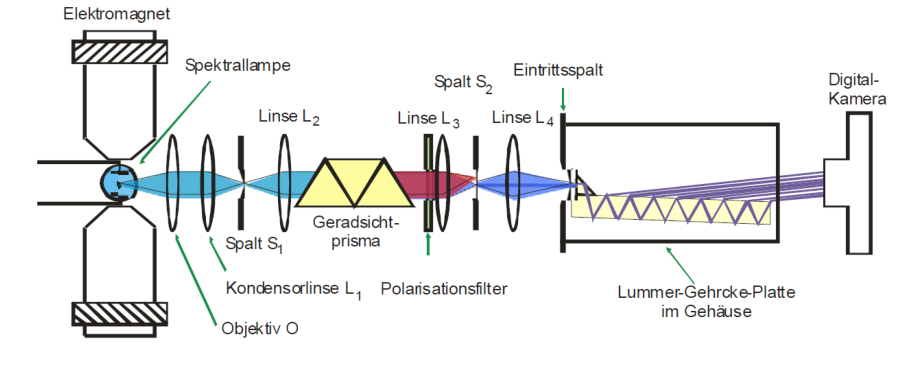
\includegraphics[width=0.7\textwidth]{latex/images/Aufbau.PNG}
    \caption{Der schematische Versuchsaufbau zur Untersuchung des Zeeman-Effekts \protect \cite{V27}.}
    \label{img:aufb}
\end{figure}
Der Aufbau des Versuchs ist in Abbildung \autoref{img:aufb} schematisch dargestellt.\\
Auf der linken Seite ist eine $\ce{Cd}$-Spektrallampe zwischen den Polen eines Magneten dargestellt. 
Wenn aktiviert sendet diese einen Strahl aus, welcher anschließend von zwei Linsen entlang des Strahlengangs gebündelt und auf einen Spalt fokussiert wird.
Nach dem Spalt wird der Strahl wieder parallelisiert und mit Hilfe eines Geradsichtprismas in seine Frequenzen aufgeteilt.
Diese durchlaufen einen Polarisationsfilter, welcher die lineare- oder zirkulare-Polarisation des Lichts herausfiltert.
Anschließend wird der Strahl so gebündelt, dass mit einem verschiebbaren Spalt eine der aufgespaltenen Farben gewählt werden kann. 
Zuletzt wird der Strahl auf das Eintrittsprisma der Lummer-Gehrcke-Platte fokussiert.\\
Diese erzeugt ein Interferenzmuster über das Vielfache reflektieren des Lichts im Inneren der Platte.
Sie besteht aus einer Platte der Dicke $d$ und Länge $l$. 
Das einfallende Strahlenbündel wird von der oberen und unteren Grenzfläche der Platte immer wieder fast vollständig reflektiert.
Allerdings tritt an der oberen Grenzschicht immer ein kleiner Teil des Strahls in Richtung einer Kamera aus. 
Dieser interferiert dort mit den anderen Strahlen, welche eine Reflexion später ausgetreten sind und somit einen kleinen Laufzeitunterschied besitzen.
Diese Funktionsweise ist schematisch in Abbildung \autoref{img:platte} dargestellt.
\begin{figure}[h]
    \centering
    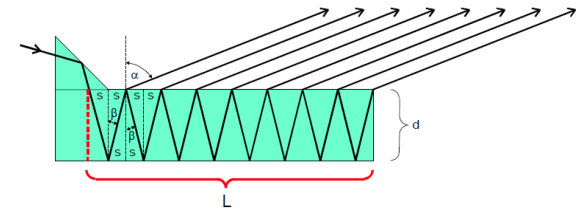
\includegraphics[width=0.7\textwidth]{latex/images/Platte.PNG}
    \caption{Die Funktion einer Lummer-Gehrcke-Platte schematisch dargestellt.\protect \cite{V27}.}
    \label{img:platte}
\end{figure}

\noindent
Für den Gangunterschied der Beugungsmaxima $m$-ter Ordnung ergibt sich dabei als Bedingung
\begin{equation}
    2nd \cos (\beta) = m \lambda \quad ,
    \label{eqn:platte}
\end{equation}
wobei $n$ der Brechungsindex der Platte ist, $\beta$ der Refletionswinkel innerhalb der Platte und $\lambda$ die Wellenlänge des Strahlenbündels.\\
Dabei ist zu beachten, dass der Gangunterschied direkt von der Wellenlänge $\lambda$ des Lichts abhängt.
Damit sich unterschiedliche Ordnungen nicht überlagern, lässt sich ein Dispersionsgebiet $\increment \lambda_\t{D}$ für die Wellenlängen bestimmen, 
in welchem die Messung möglich ist.
Für dieses gilt
\begin{equation}
    \increment \lambda_\t{D} = \frac{\lambda^2}{2d}\frac{1}{\sqrt{n^2 -1}} \quad .
\end{equation} 
Dies führt auch zum Auflösevermögen der Platte mit 
\begin{equation*}
    A = \frac{\lambda}{\increment \lambda} = \frac{L}{\lambda} (n^2 -1) \quad .
\end{equation*}


\noindent
Für die \textbf{Durchführung} wird zuerst die Stärke des Elektromagneten ausgemessen. 
Dafür wird eine Hall-Sonde zwischen die Magnetpole eingebracht und anschließend in $\increment I = \SI{0.5}{\ampere}$ 
Schritten bis zum Maximum hochgeregelt und anschließend wieder hinunter. Dabei werden die korrespondierenden Stärken des Magnetfeldes notiert.\\
Anschließend wird die Spektrallampe wieder zwischen den Magnetpolen platziert werden.
Nun wird der Aufbau so verstellt, dass die rote Wellenlänge mit $\lambda_\t{rot} = \SI{643.8}{\nano\metre}$ \cite{V27} Interferenzmuster auf der Kamera erzeugt.
Dies wird mit der Kamera aufgenommen. Des Weiteren wird dies für die lineare Polarisation mit angeschaltetem Magnetfeld wiederholt.\\
Für die blaue Wellenlänge mit $\lambda_\t{blau} = \SI{480}{\nano\metre}$ \cite{V27} wird das ganze wiederholt. 
Dabei werden die Interferenzmuster zuerst für beide Polarisationen ohne Magnetfeld aufgenommen und anschließend noch einmal für beide mit Magnetfeld.